%%%%%%%%%%%%%%%%%%%%%%%%%%%%%%%%%%%%%%%%%%%%%%%
%%%This is a science homework template. Modify the preamble to suit your needs. 
%The junk text is   there for you to immediately see how the headers/footers look at first 
%typesetting.

\documentclass[12pt]{article}

%AMS-TeX packages
\usepackage{amssymb,amsmath,amsthm} 
\usepackage{commath}
\usepackage[margin=1in]{geometry}
\usepackage{graphicx,ctable,booktabs}
\usepackage[retainorgcmds]{IEEEtrantools}
\usepackage{cancel}
\usepackage{wrapfig}
\usepackage{braket}
\usepackage{enumitem}
\usepackage{pdfpages}
\usepackage{subcaption}
\usepackage{xurl}

\usepackage{graphicx}
\usepackage{subfig}

%Redefining sections as problems

\makeatletter
\newenvironment{problem}{\@startsection
	{section}
	{1}
	{-.2em}
	{-3.5ex plus -1ex minus -.2ex}
	{2.3ex plus .2ex}
	{\pagebreak[3]%forces pagebreak when space is small; use \eject for better results
		\large\bf\noindent{Problem }
	}
}
{%\vspace{1ex}\begin{center} \rule{0.3\linewidth}{.3pt}\end{center}}
	\begin{center}\large\bf \ldots\ldots\ldots\end{center}}
\makeatother

%Fancy-header package to modify header/page numbering 

\usepackage{fancyhdr}
\pagestyle{fancy}
\lhead{Problem \thesection}
\chead{} 
\rhead{\thepage} 
\lfoot{\small\scshape PHYS 600} 
\cfoot{} 
\rfoot{\footnotesize HW 4} 
\renewcommand{\headrulewidth}{.3pt} 
\renewcommand{\footrulewidth}{.3pt}
\setlength\voffset{-0.25in}
\setlength\textheight{648pt}
\allowdisplaybreaks

\newcommand{\partder}[3]{\ensuremath{\left(\frac{\partial {#1}}{\partial {#2}}\right)_{#3}}}

\newcommand{\braks}[1]{\ensuremath{\left\langle{#1} \right\rangle} }

\newcommand{\Omx}[1]{\ensuremath{\Omega_\mathrm{#1} } }
\newcommand{\rhox}[1]{\ensuremath{\rho_\mathrm{#1} } }

\setlength{\parindent}{0pt} % No indent by default

%%%%%%%%%%%%%%%%%%%%%%%%%%%%%%%%%%%%%%%%%%%%%%%

%
%Contents of problem set
%    

\begin{document}
	
	\title{PHYS 600: Homework 4}
	\author{Yarone Tokayer}
	\date{October 27, 2023}
	
	\maketitle
	
	\thispagestyle{empty}

	\begin{problem}{Recombination}
		\begin{enumerate}
			\item hi

		\end{enumerate} 
	\end{problem}
	
	\begin{problem}{``What-if'' BBN}

	\begin{itemize}
		\item hi
	\end{itemize}
		
	\end{problem}
	
	\begin{problem}{Freeze-in DM}
		\begin{enumerate}[label=(\alph*)]
			\item hi
			
		\end{enumerate}
	\end{problem}


% Appendix
%\appendix
%\section{Python code}
%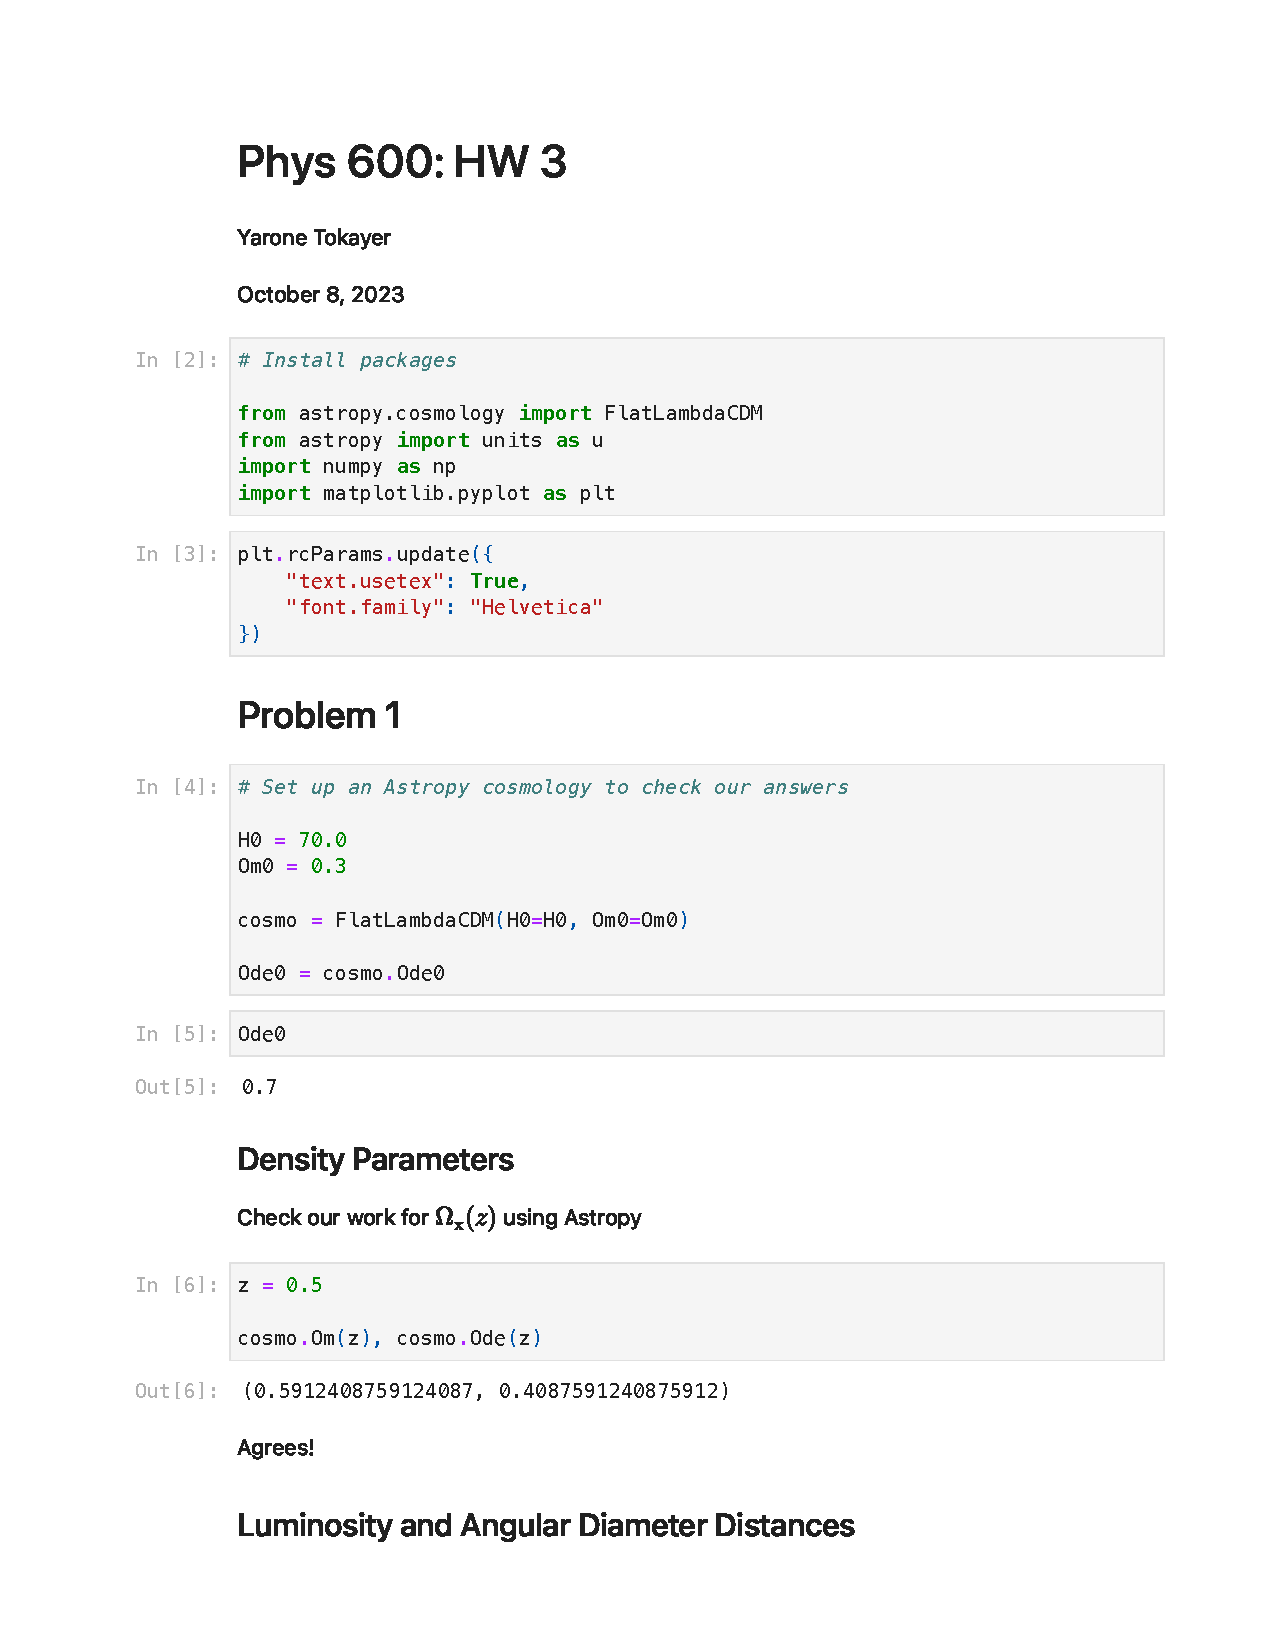
\includepdf[pages=-, frame=true, scale=0.9]{/Users/yaronetokayer/Yale Drive/Classes/PHYS 600/phys600 hw/phys600 hw 3/phys600 hw 3 work.pdf}
%\section{Mathematica code}
%
%\begin{figure}[h!]
%	\centering
%	\fbox{
%		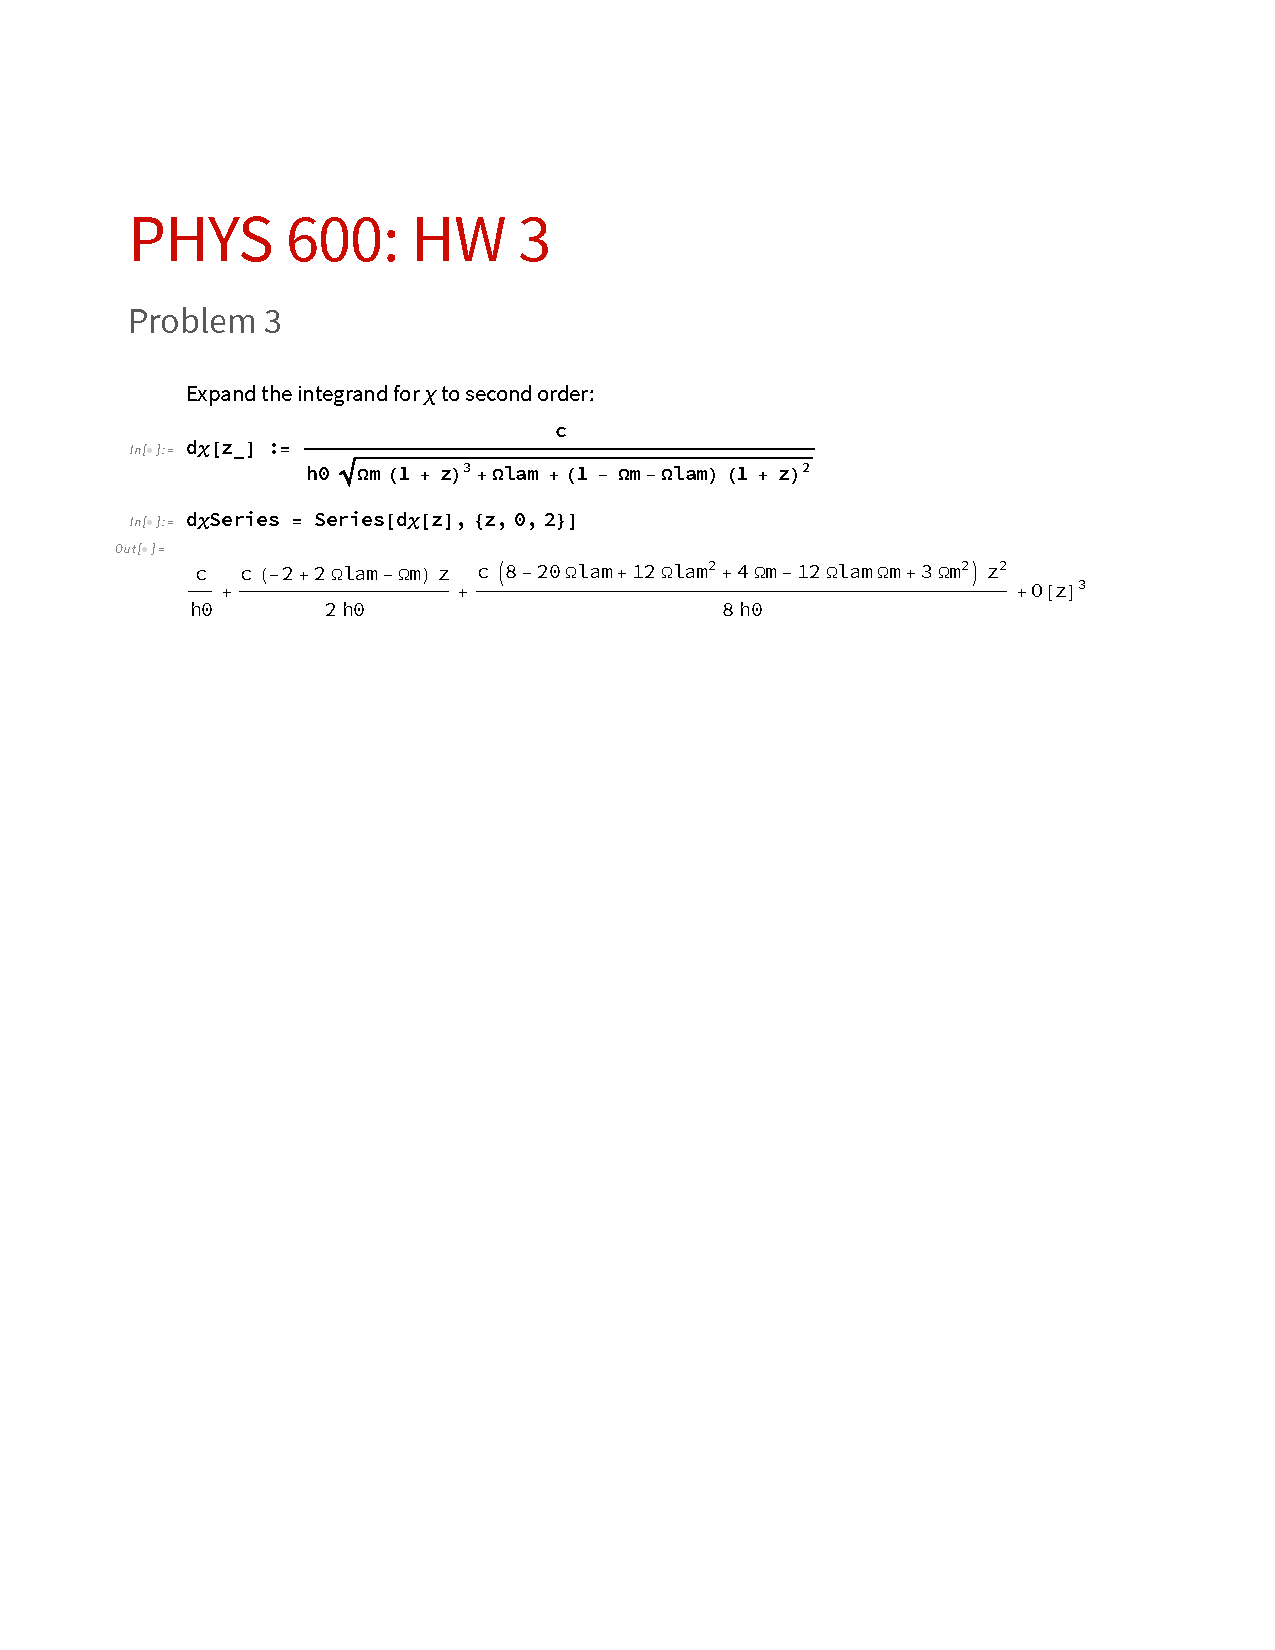
\includegraphics[trim={0 15cm 0 2cm},clip, width=0.95\linewidth]{phys600 hw 3 work nb.pdf}
%	}
%\end{figure}


\end{document}